\documentclass[dvipsnames]{beamer}
\usepackage{lmodern}
\usepackage{appendixnumberbeamer}
\renewcommand{\sfdefault}{lmss}
\renewcommand{\ttdefault}{lmtt}
\usepackage[T1]{fontenc}
% \usepackage[utf8]{inputenc}
\setcounter{secnumdepth}{3}
\setcounter{tocdepth}{3}
\usepackage{amsmath}
\usepackage{amsthm}
\usepackage{amssymb}
\theoremstyle{definition}
\newtheorem*{defn*}{\protect\definitionname}
\providecommand{\definitionname}{Definition}
\usepackage{graphicx}
\usepackage{hyperref}
\usepackage{ulem}
\PassOptionsToPackage{normalem}{ulem}
\usepackage{caption}
\usepackage{subcaption}
\usepackage{verbatim}
\usepackage[english]{babel}
\usepackage[autostyle]{csquotes}
\usepackage{tikz}
\usetikzlibrary{arrows,intersections}
\usepackage{pgfplots}
\pgfplotsset{compat = 1.15}
\usepgfplotslibrary{fillbetween}
\usepackage{verbatim}
\usepackage{booktabs}
\usepackage{multirow}
\usepackage{array}
\usepackage{nccmath}
% \usepackage{listings}
\usepackage{mathtools}

%Bibliography style, etc.
\usepackage[citestyle=authoryear-comp,natbib, uniquename = false, url = false, doi = false, uniquelist=false]{biblatex}
\renewbibmacro{in:}{}
\AtEveryBibitem{%
  \clearfield{volume}%
  \clearfield{number}
  \clearfield{month}
  \clearfield{issn}
  \clearfield{isbn}
  \clearfield{pages}
}

%\usepackage{cleveref}
\usepackage{setspace}
\makeatletter

% Macros
\providecommand{\tabularnewline}{\\}
\newcommand{\gr}{\textcolor{ForestGreen}} 
\newcommand{\rd}{\textcolor{red}}
\newcommand{\cb}{\textcolor{CornflowerBlue}} %this is the blue color you like; simply type \cb{X} where "X" is the color you want in blue
\newcommand{\vitem}{\vfill \item} %auto-centers items in lists
\newcommand{\fall}{\ \forall} %redefines "forall" (I don't like the default spacing)
\newcommand{\frall}{\quad \forall} %a \forall separated from the main math; this is the way it usually shows up in equations
\newcommand{\exist}{\ \exists} %same as \fall, but for \exists; they have the same ugly spacing
\newcommand{\R}{\mathbb{R}} %set of real numbers
\newcommand*\bigcdot{\mathpalette\bigcdot@{.5}} %different size for cdots
% \newcommand{\argmax}{\text{arg}\max}
\newenvironment{itemframe}
    {\frame{}\itemize}
    {\itemize\frame}
\newcommand\makebeamertitle{\frame{\maketitle}}%
\newtheoremstyle{named}{}{}{\itshape}{}{\bfseries}{.}{.5em}{\thmnote{#3's }#1}
\theoremstyle{named}
\newtheorem*{prop*}{Proposition}
% \newtheorem*{corollary}{Corollary}
\newtheorem*{namedtheorem}{Theorem} %allows named theorems
\newtheorem*{nameddef}{Definition}
\newtheorem{proposition}{Proposition}
\newtheorem*{assumption}{Assumption}
\newtheorem*{namedcorollary}{Corollary}
\newtheorem*{namedlemma}{Lemma}
\newtheorem*{axiom}{Axiom}
\newtheorem*{theorem*}{Theorem}
\newtheorem*{lemma*}{Lemma}
\DeclareMathOperator*{\argmin}{argmin}
\DeclareMathOperator{\argmax}{argmax}
\DeclareMathOperator{\supp}{supp}
\DeclareMathOperator{\interior}{int}
\DeclareMathOperator{\rank}{rank}
\newcolumntype{C}[1]{>{\centering\let\newline\\\arraybackslash\hspace{0pt}}m{#1}}
\newcommand{\sbt}{\,\begin{picture}(-1,1)(-1,-3)\circle*{2}\end{picture}\ }



%formatting
\usetheme{Ilmenau}
\definecolor{MIT}{rgb}{.639,.122,.204}
\definecolor{UCLA}{rgb}{0.15294117647058825, 0.4549019607843137, 0.6823529411764706}
\definecolor{UCLA_gold}{rgb}{1, 0.8196078431372549, 0}
\usecolortheme[named=UCLA]{structure}
\setbeamercolor*{palette secondary}{fg=UCLA_gold,bg=gray!15!white}
\usecolortheme{dolphin}
\setbeamertemplate{navigation symbols}{} 
\setbeamertemplate{footline}{}{}
\setbeamertemplate{headline}{}
\setbeamertemplate{navigation symbols}{}
\mode<presentation> {}
\setbeamercolor{block title}{use=structure,fg=white,bg=RoyalBlue} %blocks (theorems, etc.)in blue
\setbeamercolor{block title alerted}{use=structure,fg=white,bg=ForestGreen} %blocks (theorems, etc.)in blue

\renewcommand\qedsymbol{$\blacksquare$} %set QED symbol as black square
\renewcommand{\emph}{\textit} %set emphasized text style; this is italics
\setbeamertemplate{footline}[frame number] %slide numbers
\setbeamertemplate{itemize item}[circle] %bullet style
\setbeamertemplate{itemize subitem}{--}
\setbeamertemplate{enumerate item}[default]
\newrobustcmd*{\parentexttrack}[1]{%
  \begingroup
  \blx@blxinit
  \blx@setsfcodes
  \blx@bibopenparen#1\blx@bibcloseparen
  \endgroup}

\AtEveryCite{%
  \let\parentext=\parentexttrack%
  \let\bibopenparen=\bibopenbracket%
  \let\bibcloseparen=\bibclosebracket}

 \AtBeginDocument{%
   \let\origtableofcontents=\tableofcontents
   \def\tableofcontents{\@ifnextchar[{\origtableofcontents}{\gobbletableofcontents}}
   \def\gobbletableofcontents#1{\origtableofcontents}
 }
\newcommand{\backupbegin}{
   \newcounter{framenumberappendix}
   \setcounter{framenumberappendix}{\value{framenumber}}
}
\newcommand{\backupend}{
   \addtocounter{framenumberappendix}{-\value{framenumber}}
   \addtocounter{framenumber}{\value{framenumberappendix}} 
} 

\renewcommand{\maketitle}{
\setbeamertemplate{footline}{} 
\begin{frame}[noframenumbering]
\titlepage
\end{frame}
\setbeamertemplate{footline}[frame number]
}

\usefonttheme[onlymath]{serif}

% \usetheme{CambridgeUS}

% \newtheorem{theorem}{Theorem}
% \theoremstyle{claim}
\newtheorem{claim}{Claim}
% \newtheorem{corollary}{Corollary}


\makeatother


%\author{Drew Fudenberg}

\institute[]{}
\newcommand{\var}{\operatorname{var}}
\title{Intergenerational Mobility in American History (Ward, WP)}
\author{Chris Ackerman}
\begin{document}
\maketitle
\begin{frame}{Overview}
  \begin{itemize}
  \item \emph{Research Question:} Existing research shows that relative mobility has declined for the last 150 years. Is this true?
  \vitem \emph{Problem 1:} Long-run mobility estimates only use data on white people.
  \vitem \emph{Problem 2:} Parental status is measured with error.
  \vitem \emph{Findings:} There is more equality of opportunity now than ever before (but largely because there was a ton of inequality to start with).
  \end{itemize}
\end{frame}
%
\begin{frame}{Adding Data on Black Mobility}
  \begin{itemize}
  \item Most existing studies look only at white people
    \vfill
    \begin{quote}
      Other studies take advantage of income data from early 20$^\text{th}$ century Iowa, but Iowa was 99 percent white at the time.
    \end{quote}
    \vfill
    \begin{quote}
      Therefore, the documented decline in relative mobility is actually a decline in \emph{white} mobility. An undisputed pattern throughout history is that black sons had limited opportunities to advance, which suggests that overall mobility was not that high (Collins and Wanamaker forthcoming).
    \end{quote}
  \end{itemize}
\end{frame}
%
\begin{frame}{Data---Adding observations}
  \begin{itemize}
  \item Ignoring enslaved children from the 1850 or 1860 censuses fails to capture the impact of emancipation.
    \begin{enumerate}
    \vitem Add Southern-born Black adults from the 1870 and 1880 censuses
      \vitem Link fathers to a second (and sometimes third) observation
    \end{enumerate}
    \vitem This linking procedure throws out a lot of data, and the Black observations need to be over-weighted to match the Black share of the population.
    \vitem As long as this subsample is representative, this isn't a problem.
  \end{itemize}
\end{frame}
%
\begin{frame}{Data---Measuring Status}
  \begin{itemize}
  \item Song Score
    \begin{itemize}
    \item Occupations in a given birth cohort are percentile ranked based on their average human capital level
      \vitem Results in a 0--100 score that is merged into the linked sample
      \vitem Captures time-varying changes to relative status
    \end{itemize}
    \vitem Adjusted Song Score
    \begin{itemize}
    \item Aim is to address racial and regional inequality
      \vitem Percentile rank an occupation, race, and region's literacy rate/educational level
      \begin{itemize}
      \item For example, in the 1850s, 96 percent of white farmers in the North were literate, 85 percent of white farmers in the South, and 44 percent of Black farmers in the South
      \end{itemize}
    \end{itemize}
  \end{itemize}
\end{frame}
%
\begin{frame}{Measuring Intergenerational Mobility}
  \begin{itemize}
  \item Focus on \emph{relative mobility}, which is whether a father's place in the economic distribution matters for the child's place.
    \vitem Most common relative mobility estimates come from regressing the son's outcome $y_{i, s}$ on the father's outcome, $y_{i, f}$:
    \[
y_{i, s} = \beta_0 + \gr{\beta_1} y_{i, f} + \varepsilon_{i, s}
    \]
  \end{itemize}
\end{frame}
%
\begin{frame}{Within-Between Decomposition of $\gr{\beta_1}$}
  \[
\hat{\beta}_1 = \underbrace{\sum^G_{g = 1} \textcolor{blue}{\theta^g}\hat{\beta}^g_1}_{\text{within group}} + \underbrace{\rd{\theta^b}\hat{\beta}^b_1}_{\text{between group}}
  \]
  \begin{itemize}
  \item $\textcolor{blue}{\theta^g}$ is the share of variation in the father's status from within-group (white or black)
    \vitem $\rd{\theta^b}$ is the share of variation between group means
  \end{itemize}
\end{frame}
%
\begin{frame}{Accounting for Measurement Error (overview)}
  \begin{itemize}
  \item Existing research often only looks at a single-year snapshot of paternal ``status'', but we have evidence that job data is recorded with \emph{considerable} error.
    \vitem The best way to overcome this measurement error is to average over multiple observations, when data are available.
    \vfill
    \begin{quote}
      This instability influences mobility estimates: for a sample of white families, going from one snapshot to averaging three father observations increases the father-son association of status by 27 to 32 percent\ldots Assuming classical measurement error, eliminating noise leads to ``true'' father-son associations that are 45 to 56 percent higher than when using one observation.
    \end{quote}
  \end{itemize}
\end{frame}
%
\begin{frame}{Accounting for Measurement Error (theory)}
  \begin{itemize}
  \item Assume there is classical measurement error; a parent's income varies from permanent income by random noise,
    \[y_{i, f} = y_{i, f}^\ast + \nu_{i, f}\]
    \vitem Attenuation bias falls when we average the father's income over more time periods $T$,
    \[
\operatorname{plim}\widehat{\beta_{\text{avg}}} = \beta_1 \frac{\var(y^\ast_{i, f})}{\var (y^\ast_{i, f}) + \rd{\frac{\var(\nu_{i, f})}{T}}}
    \]
    \vitem Modern-day studies use long-run averages of ten or fifteen years
    \vitem Historical data rarely go beyond $T = 1$ due to the high costs of linking censuses
  \end{itemize}
\end{frame}
%
\begin{frame}{Accounting for Measurement Error-Does it matter?}
  \begin{figure}[htp]
    \centering
    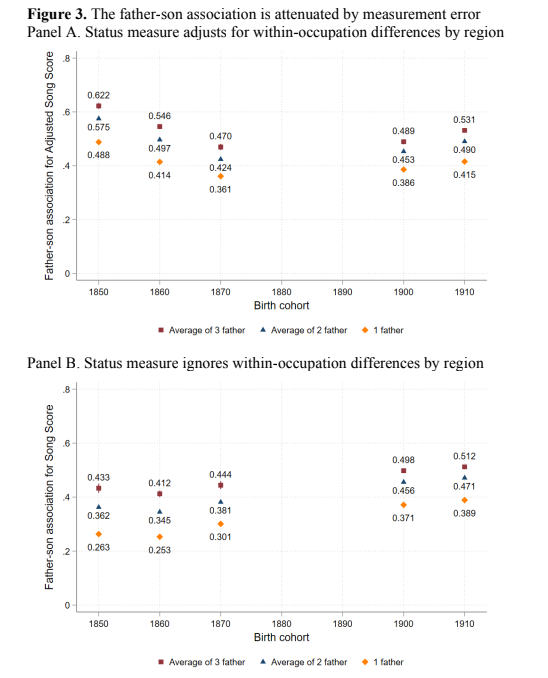
\includegraphics[height=0.9\textheight, keepaspectratio=true]{ward_fig3.png}
  \end{figure}
\end{frame}
%
\begin{frame}{Results---Adjusting mobility estimates}
  \begin{itemize}
  \item First, use IV to get around classical measurement error problem.
    \begin{itemize}
    \item Estimates imply that only 27--49 percent of gaps across white families disappeared in the next generation; America not so mobile
    \end{itemize}
  \vitem Now account for racial persistence
    \begin{itemize}
    \item Initial estimates are only for white males, $\hat{\beta}_1^{\text{white}}$
    \vitem Recall the within-between decomposition,
      \[
\hat{\beta}_1 = \theta^\text{white}\hat{\beta}_1^\text{white} + \theta^\text{Black}\hat{\beta}_1^\text{black} + \theta^b  \hat{\beta}^b_1
\]
\vitem Now estimate $\hat{\beta}_1$, which will result in a different estimate if within-Black persistence $\hat{\beta}_1^\text{Black}$ is different from within-White persistence, or if between-race persistence $\hat{\beta}^b_1$ is strong
    \end{itemize}
  \end{itemize}
\end{frame}
%
\begin{frame}{Results---Adjust mobility estimates}
  \begin{figure}[htp]
    \centering
    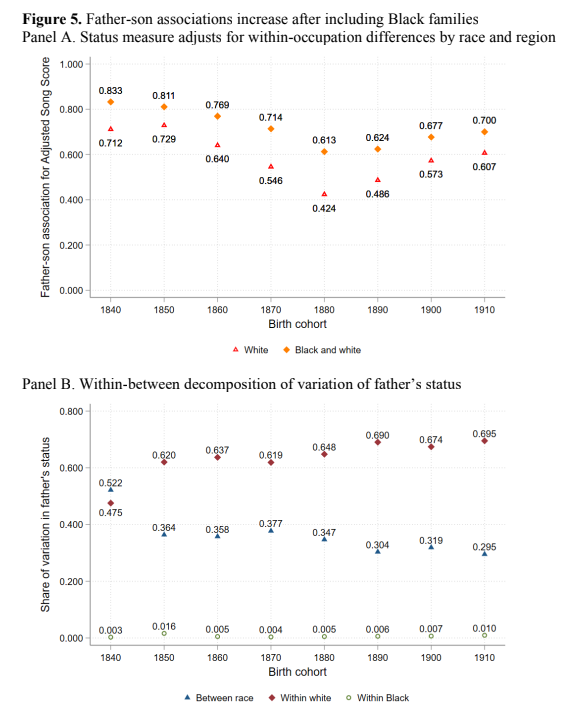
\includegraphics[height=0.9\textheight, keepaspectratio=true]{ward_fig5.png}
  \end{figure}
\end{frame}
%
\begin{frame}{Results---Adjust mobility estimates}
  \begin{itemize}
  \item Increase in father-son association is not because of an especially high Black association $\hat{\beta}_1^\text{black}$
    \vitem Large between-race effect explains the increase in the father-son association when pooling Black families
    \begin{enumerate}
    \vitem Between-race share of variation was high (peak of 0.52 in 1840, when  most Blacks were enslaved; settling around 0.30 in 1910)
      \vitem Between-race gaps persisted at 0.87 and 1.00. About 30 percent of the historical Black and white association is due to a between-race effect
    \end{enumerate}
  \end{itemize}
\end{frame}
%
\begin{frame}{Conclusions}
  \begin{itemize}
  \item Existing mobility estimates are inaccurate because they only focus on data for white males, and ignore the relative immobility of minority groups.
    \vitem Adjusting for data composition results in \emph{lower} historical mobility estimates.
    \vitem In fact, America has more equal opportunity today than ever before.
  \end{itemize}
\end{frame}
\end{document}

%%% Local Variables:
%%% mode: latex
%%% TeX-master: t
%%% End:
